%%%%%%%%%%%%%%%%%%%%%%%%%%%%%%%%%%%%%%%%%%%%%%%%%%%%%%%%%%%%%%%%%%%%%%%%%%%%%%%%
%% SUBSECTION: Metodologia badania
%%%%%%%%%%%%%%%%%%%%%%%%%%%%%%%%%%%%%%%%%%%%%%%%%%%%%%%%%%%%%%%%%%%%%%%%%%%%%%%%
\subsection{Metodologia badania}

Podstawą badania zużycia energii jest pomiar wartości pobieranego prądu przez zestaw uruchomieniowy
P-NUCLEO-WB55 w czasie. Posiadając dane wymienione dane, na podstawie oczywistych
zależności fizycznych wyznacza się parametry jak całkowita wykorzystana energia
podczas badania, przedstawiona w przystępnej postaci parametru mocy.

Pomiary wartości chwilowego poboru prądu oparto o moduł opisany w punkcie~\ref{device:plytka_pomiarowa}.
Źródłem energii dla płytki pomiarowej jest komputer klasy PC, a precyzyjniej udostępniany
port USB. Wykorzystując również ten protokół następuje transmisja danych poprzez komunikację szeregową
UART, umożliwiając akwizycję danych.

Połączenie z zestawem uruchomieniowym oparto o konektor CN14 udostępniający piny: PIN1 - masa GND, PIN3 - VCC $3.3V$~\cite{noauthor_um2243_2018}.
Wyprowadzone przewody połączono następnie z P-NUCLEO-WB55 poprzez konektor JP2, wcześniej pozbawiony zawleczki.
Jest to metoda rekomendowana dla pomiaru prądu opisana w dokumentacji zestawu~\cite{stmicroelectronics_um2435_2019}\footnote{
Rozdział 7.12 Current measurement}. Porty kompatybilne z Arduino/ST Morpho mogłyby stanowić równorzędny sposób
włączenia zestawu uruchomieniowego do obwodu płytki pomiarowej. Autorska analiza dokumentacji sugeruje jednak,
iż opcja ta nie jest wspierana. Wymagane byłoby lutowanie dodatkowego połączenia w (punkcie SB27), by móc wykorzystać
zasilanie napięciem $3.3V$.

\begin{figure}[!htb]
	\centering 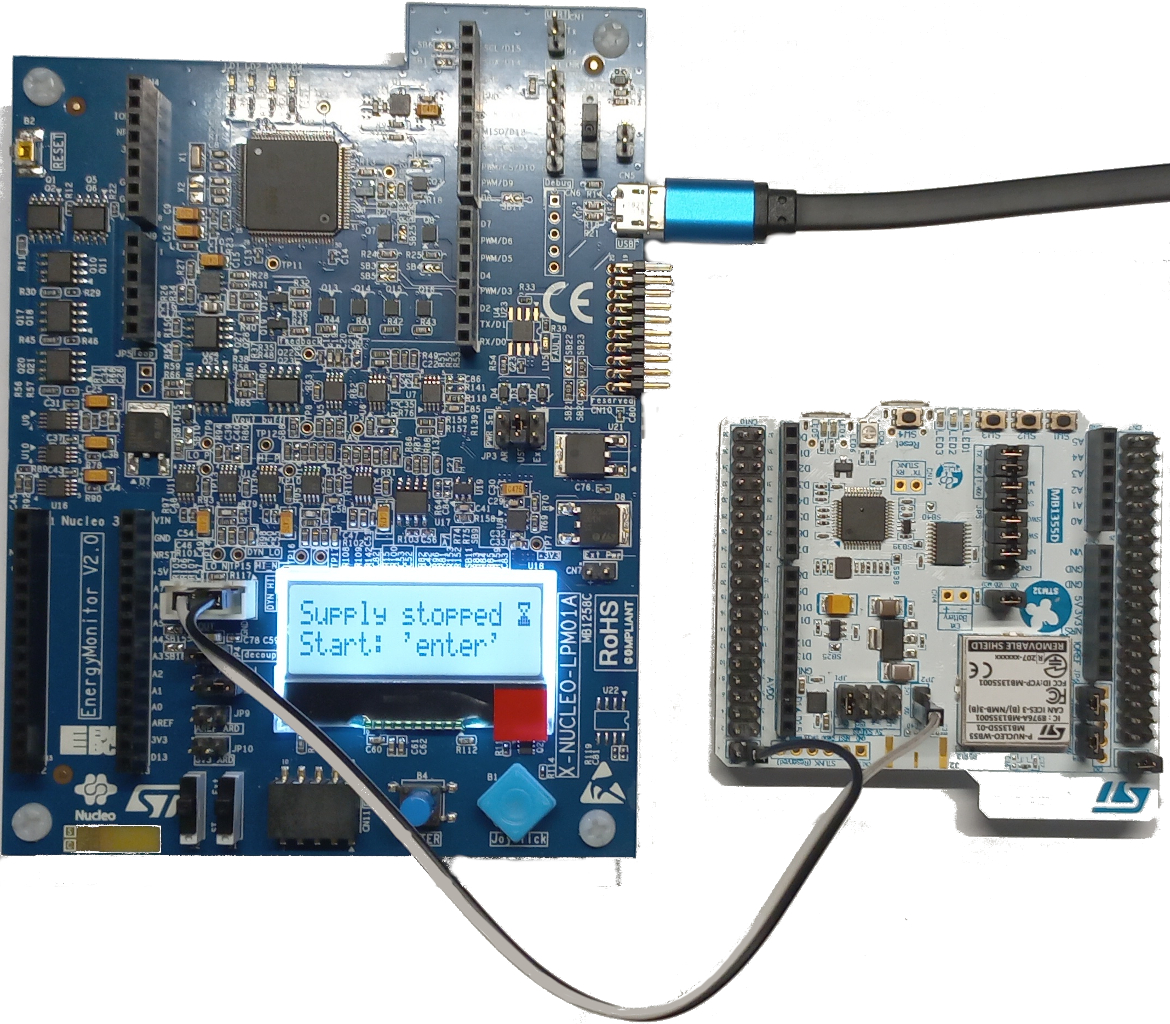
\includegraphics[width=0.618\linewidth]{power_measurement_unit_connected.png}
	\caption{Podłączony zestaw pomiarowy}
	\label{rys:connected_power_measurement_unit}
\end{figure}

Celem akwizycji danych wybrano dostarczane przez producenta oprogramowanie \textit{STM32CubeMonitor-Power}.
Pojedyncza sesja pomiarowa trwająca 100 sekund zapewnia niezbędne dane. Są one następnie
odpowiednio przetwarzane poprzez odcięcie wartości zebranych w ostatnich sekundach. Związane to było
ze sposobem działania mikrokontrolera, który po 60 sekundach domyślnie przechodzi w stan zwiększonej
oszczędności energii (Low Power Advertising). Parametr ten można zmienić wg własnych upodobań, aczkolwiek zdecydowano
się na domyślne nastawy, tak by umożliwić możliwie proste ponowne przeprowadzenie doświadczenia wykorzystując przykład
BLE HRT dostarczony przez ST. Stąd, by rozróżnić różne tryby pracy \gls{BLE}, zdecydowano o odcięciu
połowy okresu pomiarowego, zapewniając jednolite wartości względem trybów zużycia energii
w~50 sekundowym oknie.

\begin{figure}[!htb]
	\centering 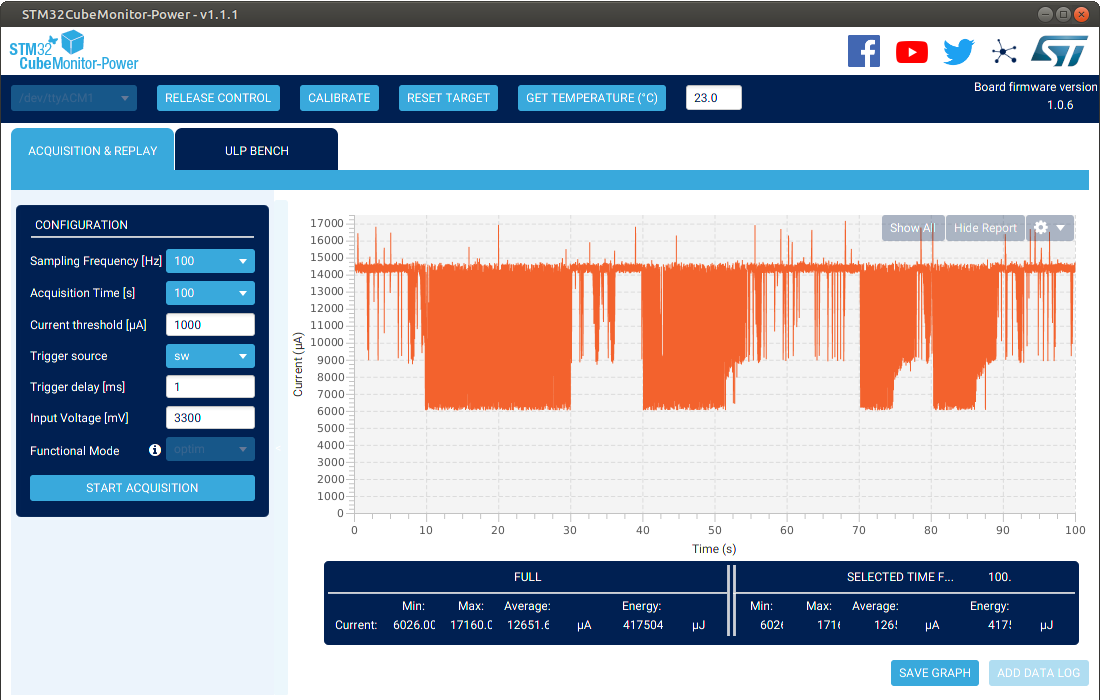
\includegraphics[width=0.99\linewidth]{stm32_power_monitor_sample.png}
	\caption{Przykładowa sesja pomiarowa dla BLE Mesh - sieć w trybie nasłuchującym}
	\label{rys:measurement_session_sample}
\end{figure}

Tak zebrane dane następnie przetworzono uzyskując wartości energii i średniej mocy
użytej przez układ. Wykorzystuje się w celu oczywistą zależność fizyczną zaprezentowaną
wzorem~\ref{energy_equation}\cite{skoro_marta_fizyka_1973}.

\begin{equation} \label{energy_equation}
E_{\text{całkowita}} = U \cdot \int_{t=0[s]}^{t=50[s]} \mathrm{d}i \: \mathrm{d} t
\end{equation}

\begin{equation} \label{power_equation}
P = \frac{E_{\text{całkowita}}}{t}
\end{equation}

gdzie:

\begin{description}
\item $E_{\text{całkowita}} [J]$ - wykorzystana energia podczas 50s sekundowej sesji rejestracji danych
\item $P [W]$ - moczużyta podczas 50s sekundowej sesji rejestracji danych
\item $U [V]$ - napięcie zasilania mikrokontrolera - 3.3V - stała
\item $\mathrm{d}i [A]$ - prąd w danej chwili
\item $\mathrm{d}t [s]$ - podstawa czasowa całkowania, 0.01s/interwał (100Hz) - stała 
\end{description}

Zebrane dane w postaci wartości chwilowych pobieranego przez mikrokontroler prądu względem czasu
przetworzono z użyciem metod numerycznych. W~celu wyliczenia łącznej wykorzystanej energii, a~tym samym
mocy, stosuje się zależność~\ref{energy_equation}. Uwzględniając fakt działania w domenie dyskretnej,
wykorzystano kompozytową metodę całkowania Simpsona~\cite{noauthor_scipyintegratesimpson_nodate}.
Podstawą dla całkowania są wartości zebrane w równoodległych odstępach. Dokonując akwizycji danych
dobrano częstotliwość próbkowania jako $100Hz$. Każda kolejna wartość charakteryzuje się więc
10 milisekundową różnicą w~podstawie czasu. Uwzględniając ten fakt, wyliczenie wartości
wykorzystanej energii jak i~mocy staje się trywialne.

%%%%%%%%%%%%%%%%%%%%%%%%%%%%%%%%%%%%%%%%%%%%%%%%%%%%%%%%%%%%%%%%%%%%%%%%%%%%%%%%
%% SUBSECTION: BT Low Energy - Usługa Heart Rate
%%%%%%%%%%%%%%%%%%%%%%%%%%%%%%%%%%%%%%%%%%%%%%%%%%%%%%%%%%%%%%%%%%%%%%%%%%%%%%%%
\subsection{BT Low Energy - Usługa Heart Rate}

Pierwszą usługą BLE badaną pod kątem zużycia energii jest Heart Rate\footnote{z ang. rytm serca}. Wybór
ten podyktowany jest chęcią przyszłego zestawienia wartości z~rozwiązaniami innych producentów.
Usługa zdefiniowana przez Bluetooth SIG stanowi więc wspólny międzyplatformowy język.
Porównanie konkurencyjnych rozwiązań względem ST stanowi potencjalny kierunek dalszych badań.

Badania przeprowadzono dla trzech różnych trybów działania aplikacji BLE HRT:
\begin{itemize}
\item Usługa połączona (Connected)
\item Usługa w trybie szybkiego ogłaszania (Fast Advertising)
\item Usługa w trybie niskomocowego ogłaszania (Low Power Advertising)
\end{itemize}

Emitowana moc ustalona została na $-0.15dBm$. Jest to wartość wspólna dla każdego pomiaru
dotyczącego BLE HRT.

Rysunek~\ref{rys:power_ble_hr_connected_only_amps} przedstawia charakterystykę poboru prądu
w czasie po ustanowieniu połączenia urządzeniem klienckim. Mikrokontroler publikuje 
losowe dane z częstotliwością $1Hz$. W konsekwencji radio zestawu uruchomieniowego
uruchamiane jest co najmniej raz na sekundę.

Analizując wykres dostrzega się regularne, 10-sekundowe interwały w których pobierany prąd dąży do swojego
maksimum wynoszącego ok. $12mA$. Jest to prawdopodobnie związane z ustawionymi parametrami transmisji
danych w mikrokontrolerze. Niniejsza praca nie podejmuje jednak próby wyjaśnienia rzeczywistej przyczyny tego zjawiska.
Minimalny zarejestrowany pobór prądu ustalony jest na ok. $422uA$, czyli o dwa rzędy wielkości mniejsze wartości
szczytowej.


\begin{figure}[!htb]
	\centering 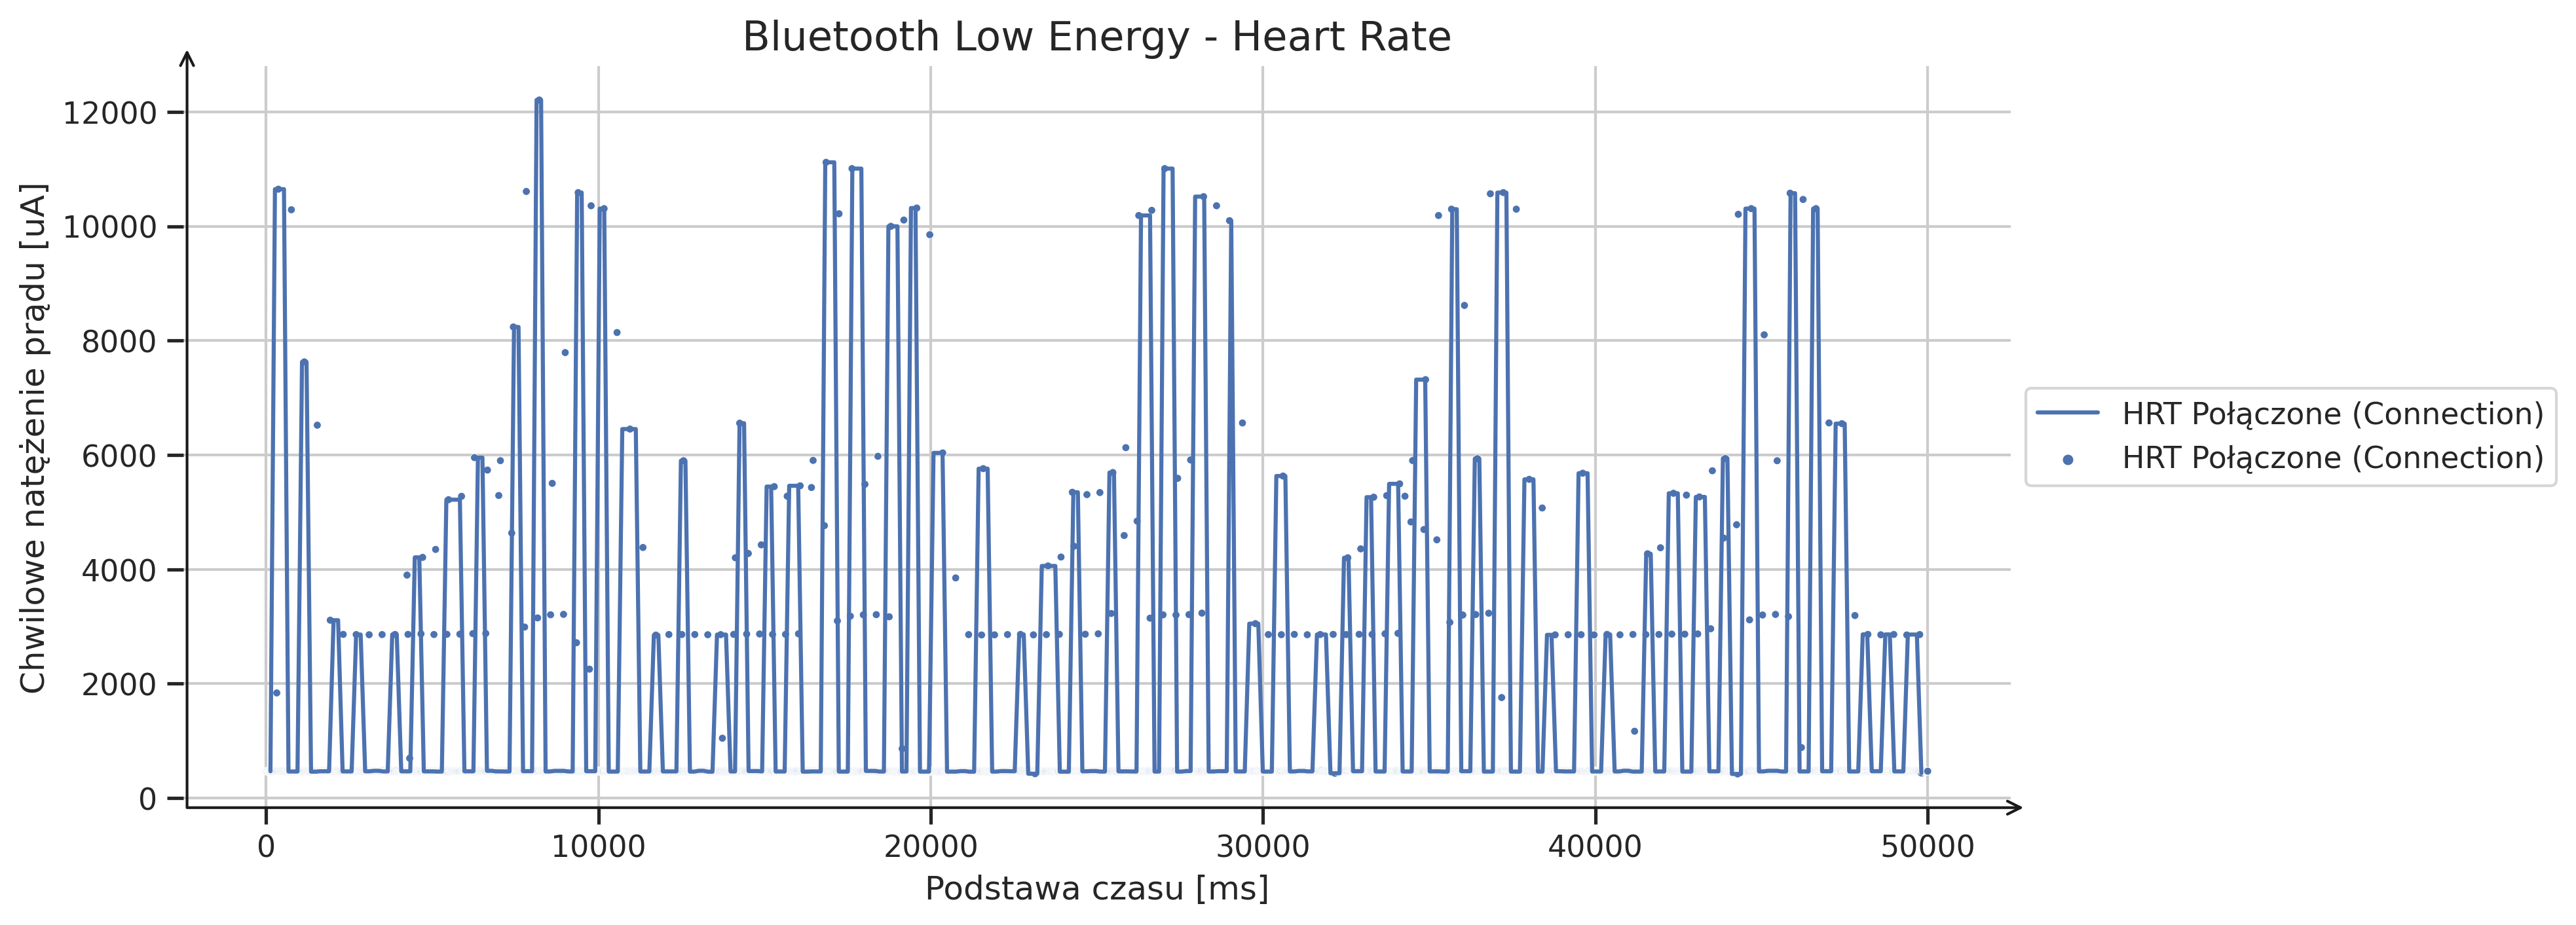
\includegraphics[width=0.99\linewidth]{power_ble_hr_connected_only_amps.png}
	\caption{Charakterystyka czasowa poboru prądu dla BLE i usługi Heart Rate - Usługa Połączona}
	\label{rys:power_ble_hr_connected_only_amps}
\end{figure}

Rysunek~\ref{rys:power_ble_hr_fastadv_only_amps} przedstawia charakterystykę poboru prądu po czasie
dla szybkiego trybu ogłoszeniowego. Zgodnie za kodem źródłowym, interwały w których rozgłaszane
są komunikaty powinny się zawierać w częstości od 80 do 100ms. Wywołuje to konieczność uruchamiania radia
co najmniej 10 razy na sekundę. Ma to swoje odzwierciedlenie na wykresie. Charakterystyka jest bardziej
\textit{burzliwa} w porównaniu z~\ref{rys:power_ble_hr_connected_only_amps}. 


\begin{figure}[!htb]
	\centering 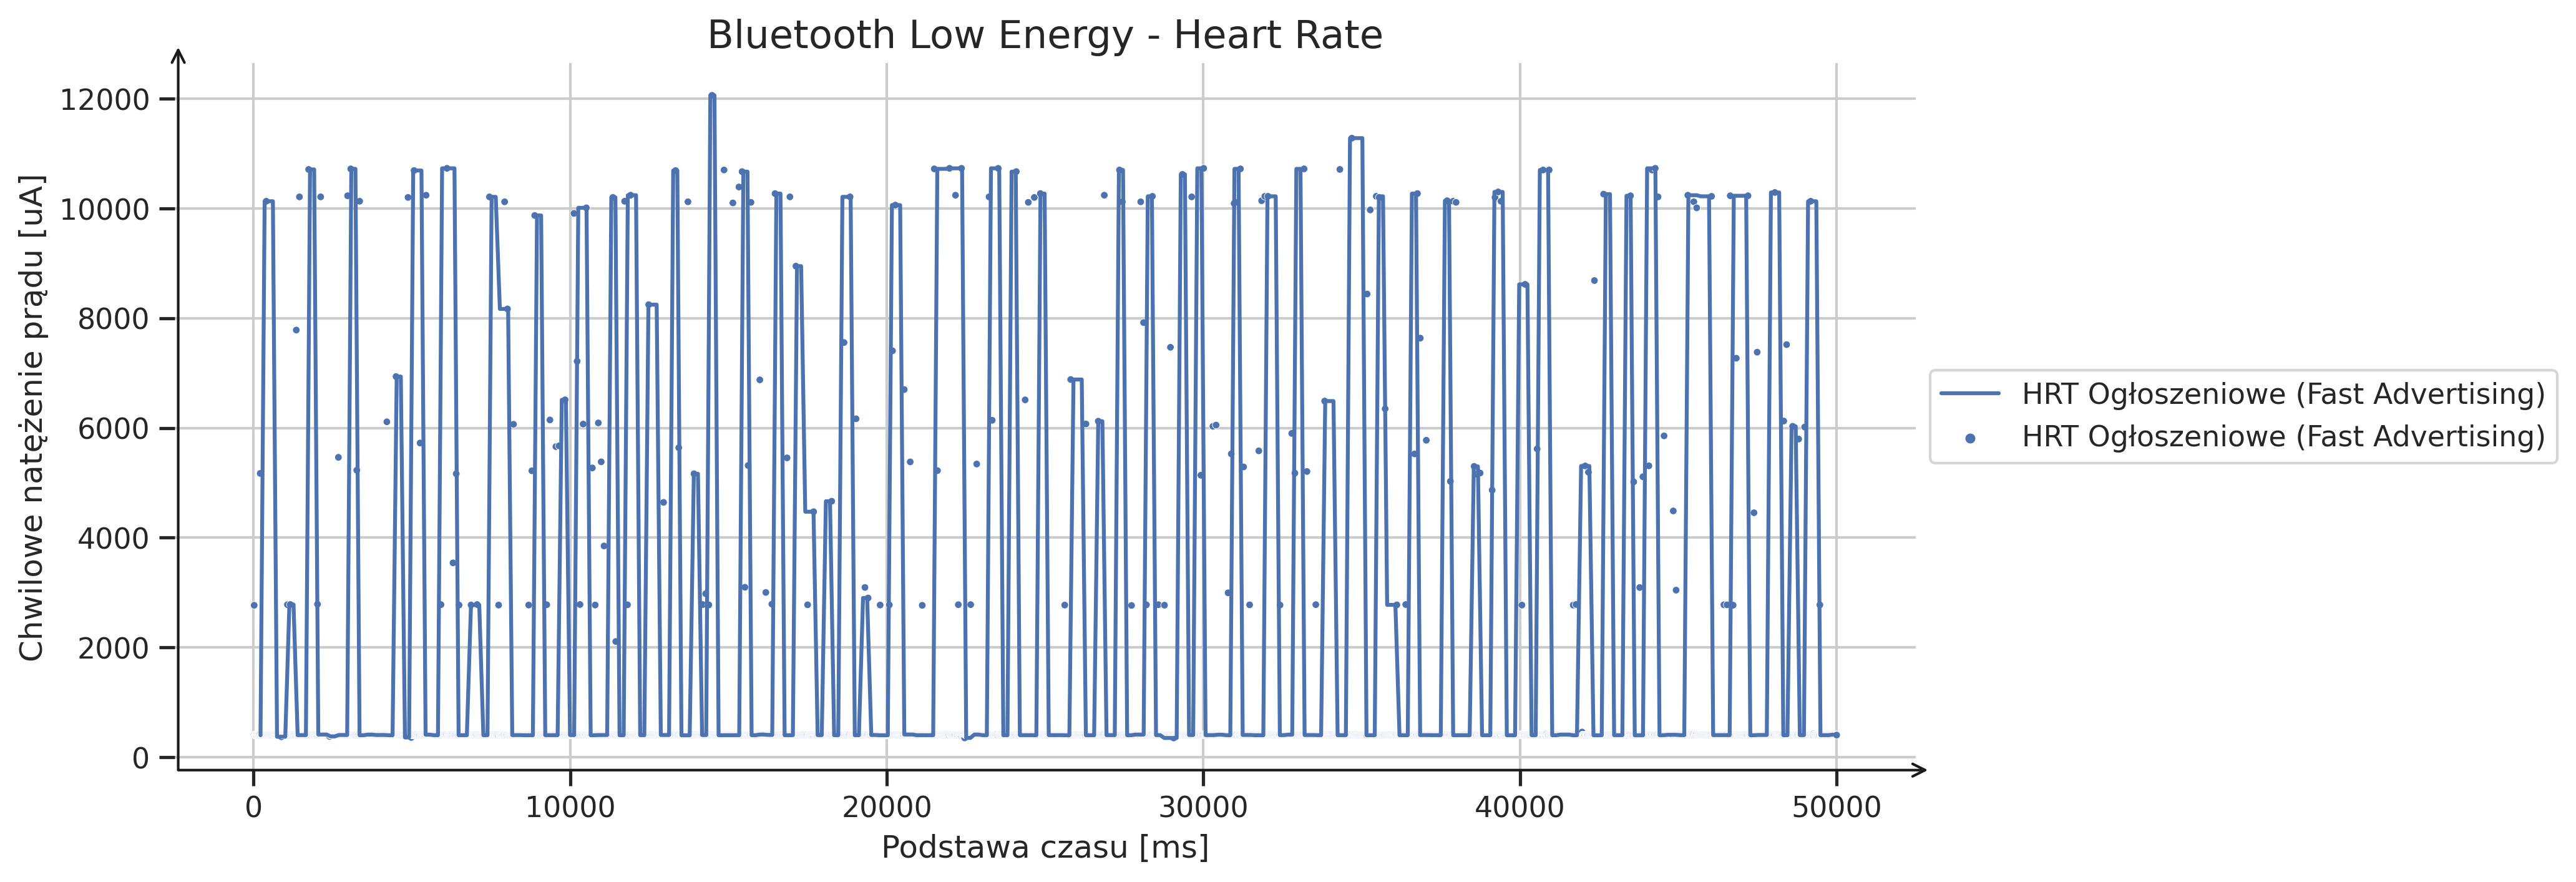
\includegraphics[width=0.99\linewidth]{power_ble_hr_fastadv_only_amps.png}
	\caption{Charakterystyka czasowa poboru prądu dla BLE i usługi Heart Rate - Tryb szybkiego ogłaszania}
	\label{rys:power_ble_hr_fastadv_only_amps}
\end{figure}

\lipsum[1-3]
\begin{figure}[!htb]
	\centering 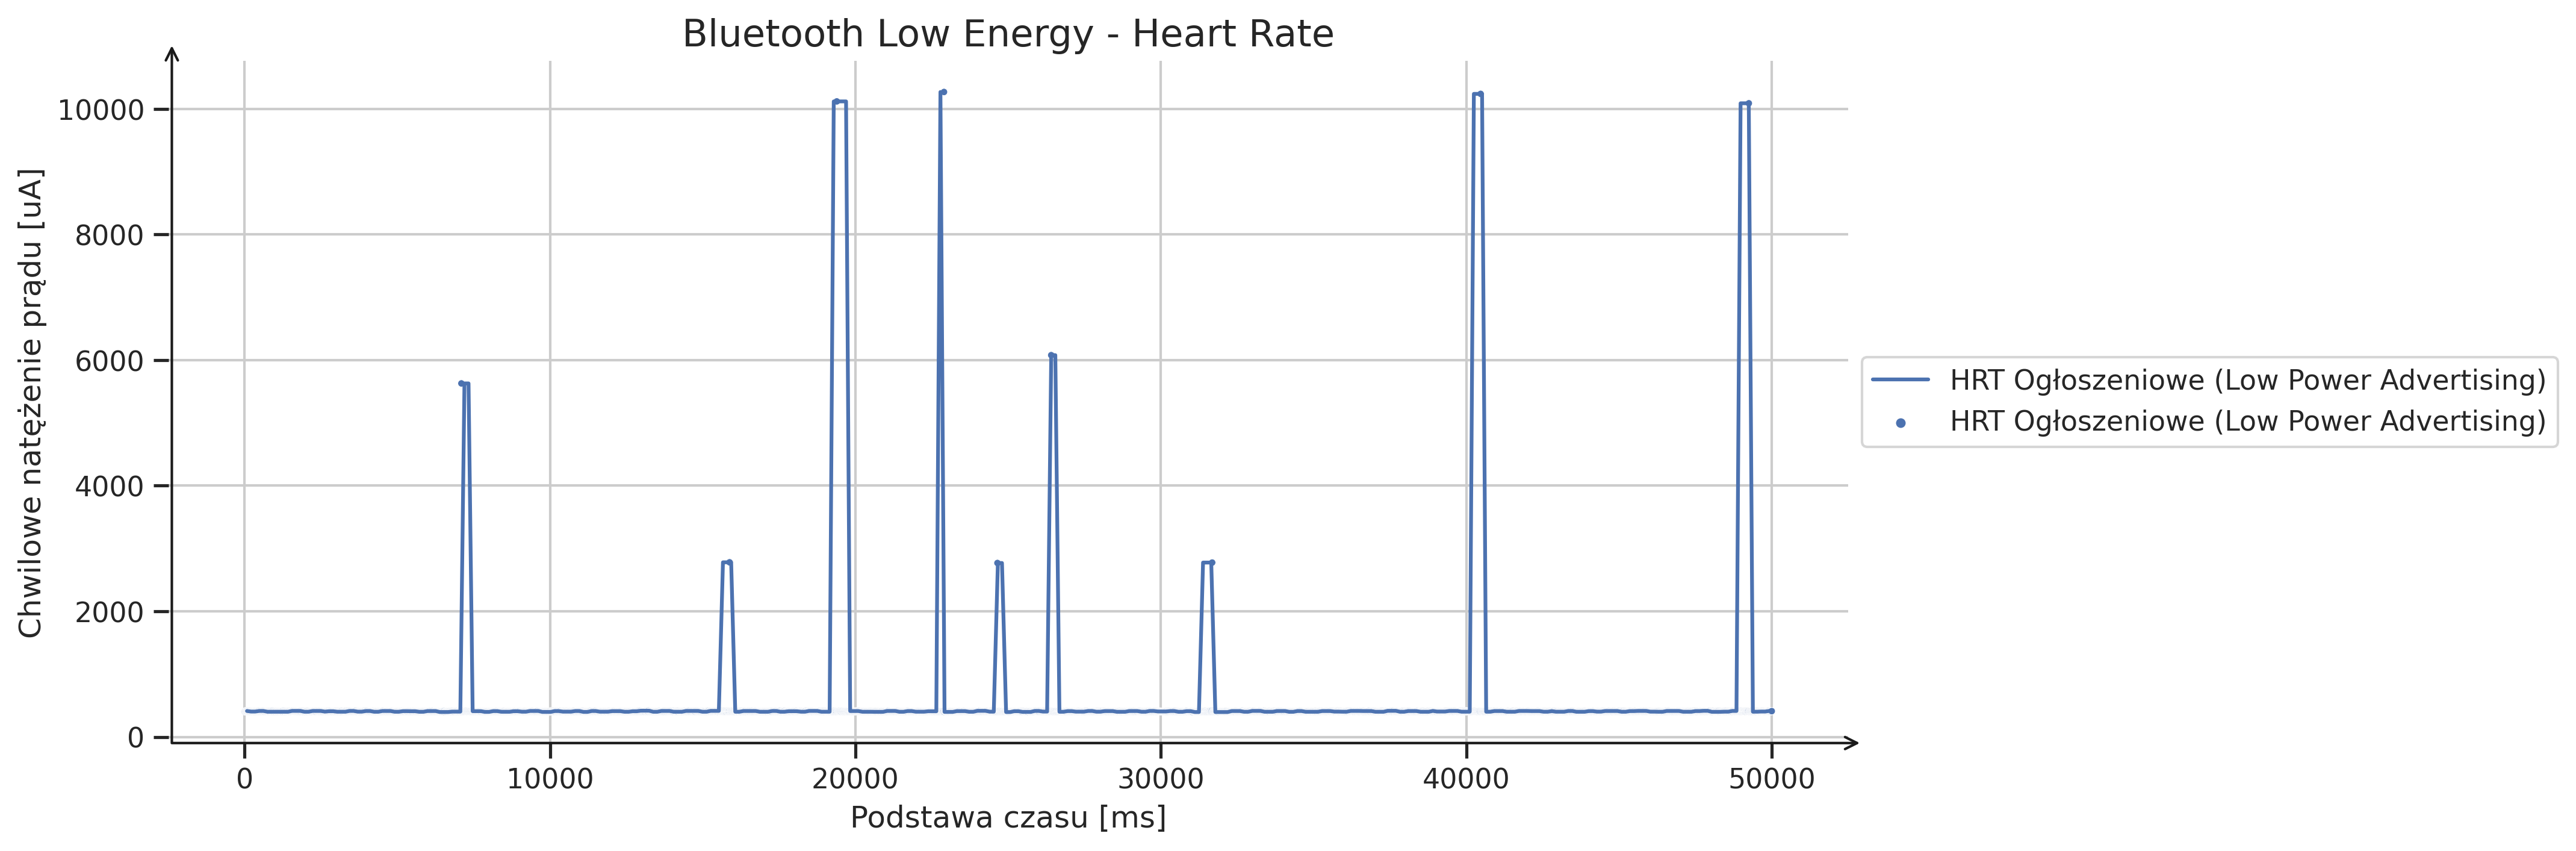
\includegraphics[width=0.99\linewidth]{power_ble_hr_low_power_adv_only_amps.png}
	\caption{Charakterystyka czasowa poboru prądu dla BLE i usługi Heart Rate - Tryb niskomocowego ogłaszania}
	\label{rys:power_ble_hr_low_power_adv_only_amps}
\end{figure}


\lipsum[1-2]
\begin{figure}[!htb]
	\centering 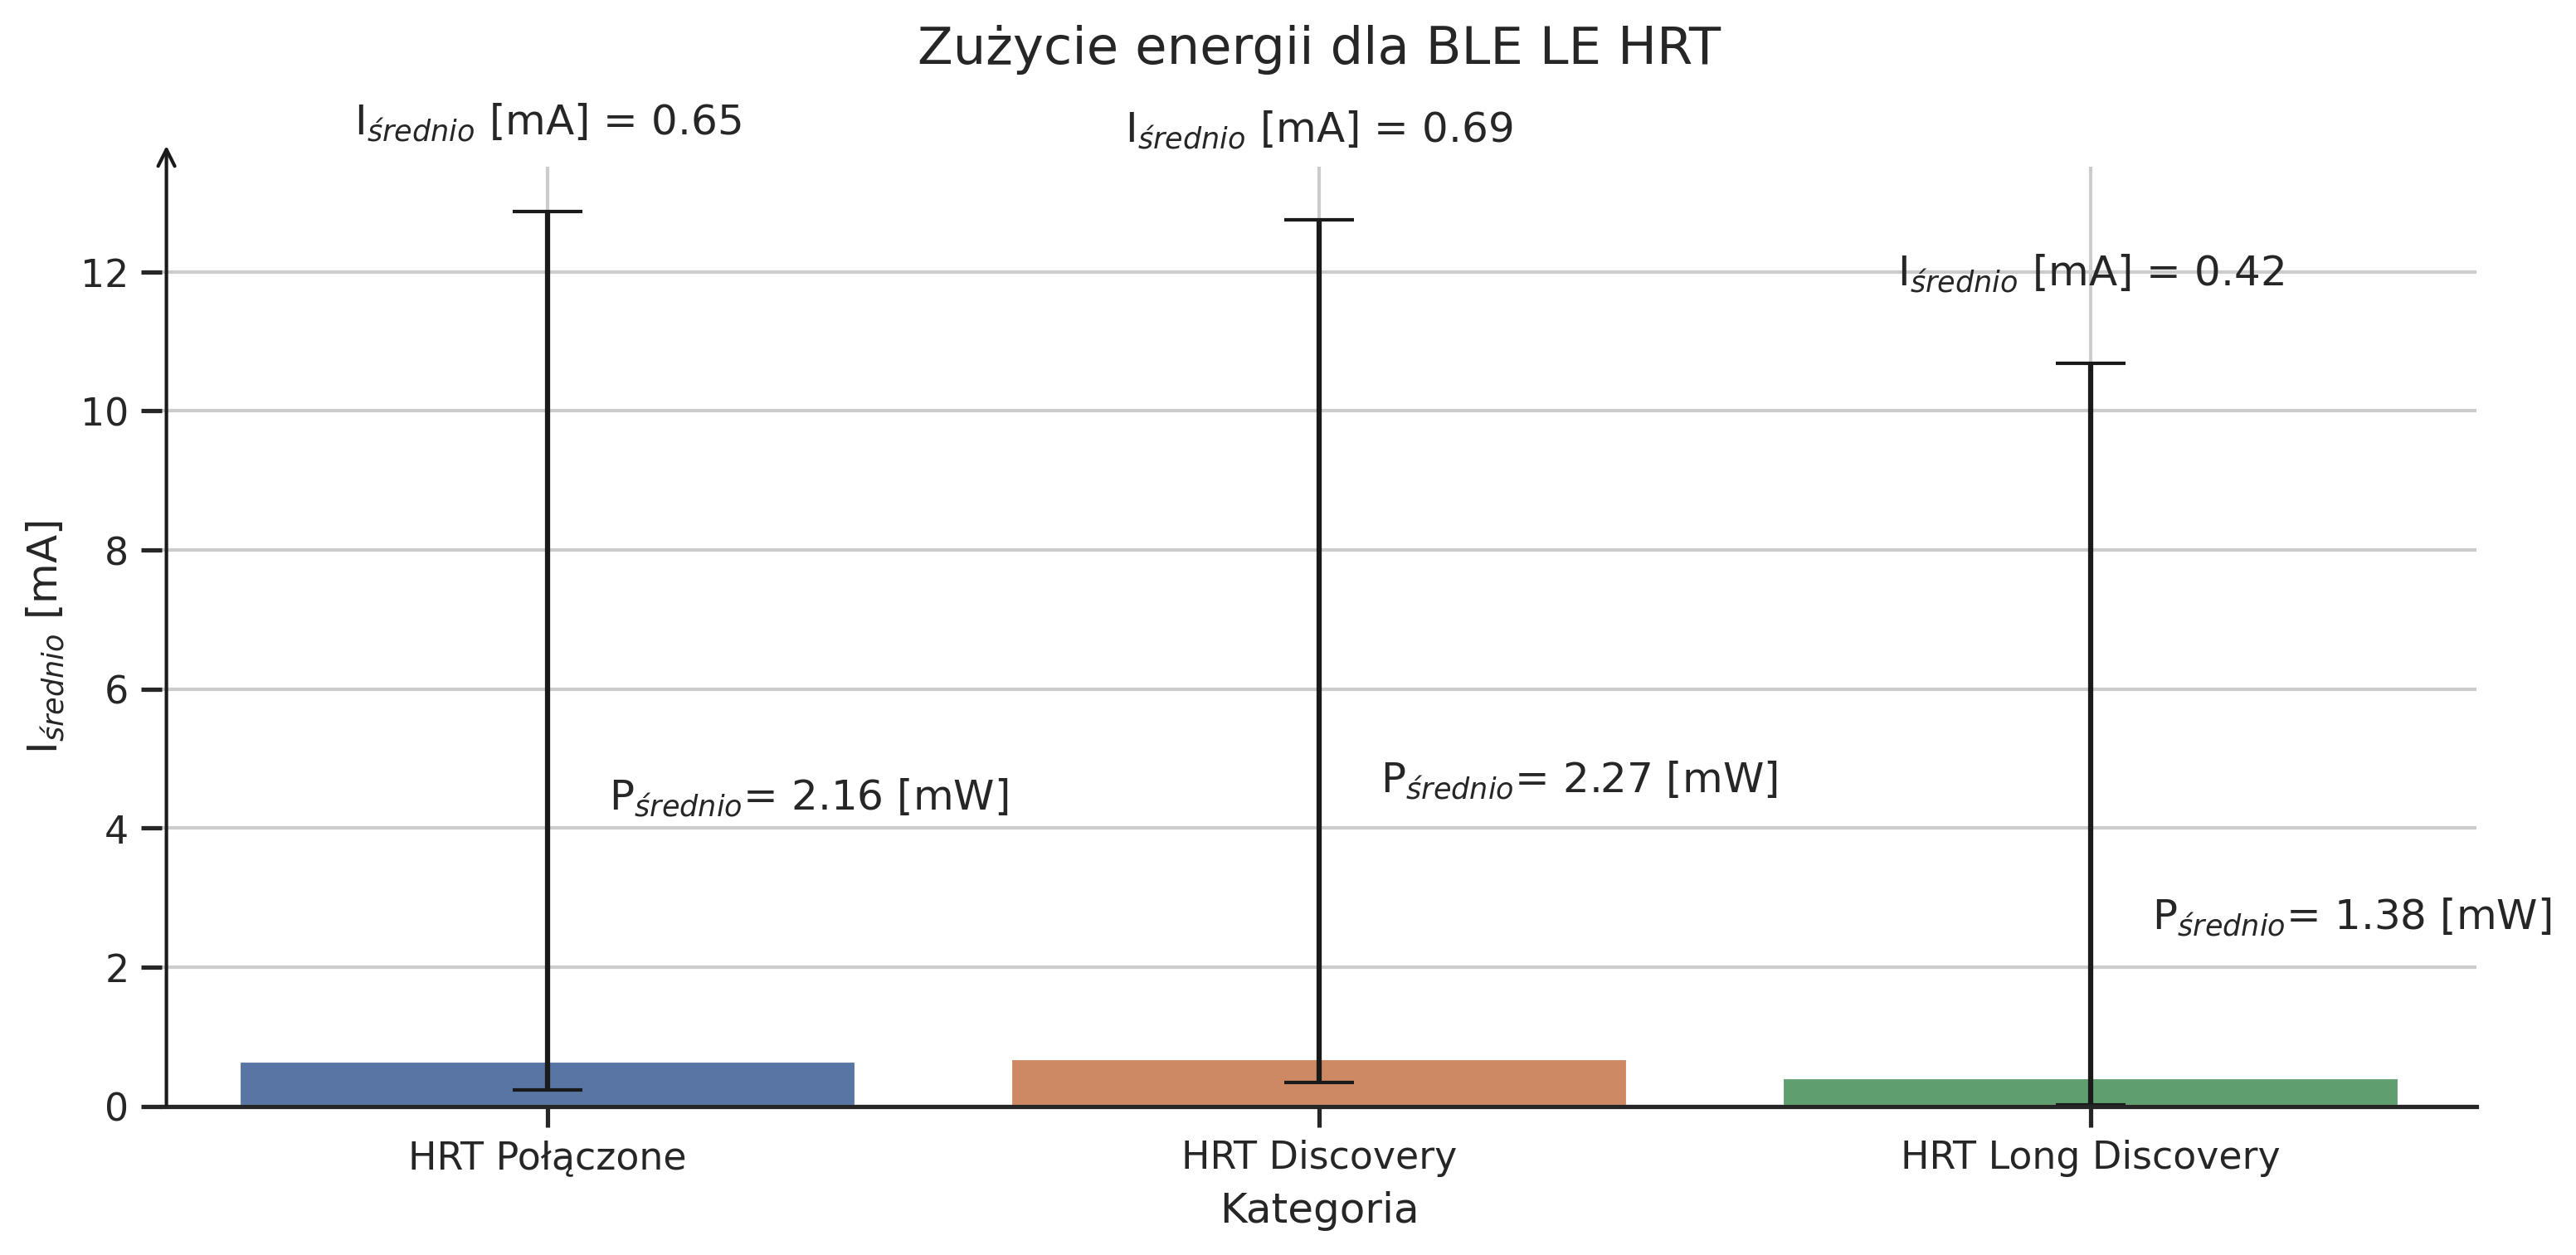
\includegraphics[width=0.99\linewidth]{power_ble_hr_amps_usage_juxtaposition.png}
	\caption{Zestawienie zużycia prądu dla usługi Heart Rate w zależności od trybu działania}
	\label{rys:power_ble_hr_amps_usage_juxtaposition}
\end{figure}
\lipsum[1-3]

%%%%%%%%%%%%%%%%%%%%%%%%%%%%%%%%%%%%%%%%%%%%%%%%%%%%%%%%%%%%%%%%%%%%%%%%%%%%%%%%
%% SUBSECTION: BLE Mesh - Model Generic OnOff
%%%%%%%%%%%%%%%%%%%%%%%%%%%%%%%%%%%%%%%%%%%%%%%%%%%%%%%%%%%%%%%%%%%%%%%%%%%%%%%%
\subsection{BLE Mesh - Model Generic OnOff}

Pomiary dla BLE Mesh uwzględniające dwa tryby działania: sieć w oczekująca na komunikaty oraz podczas działania aktywnego korzystania z Modelu Generic OnOff.

\begin{figure}[!htb]
	\centering 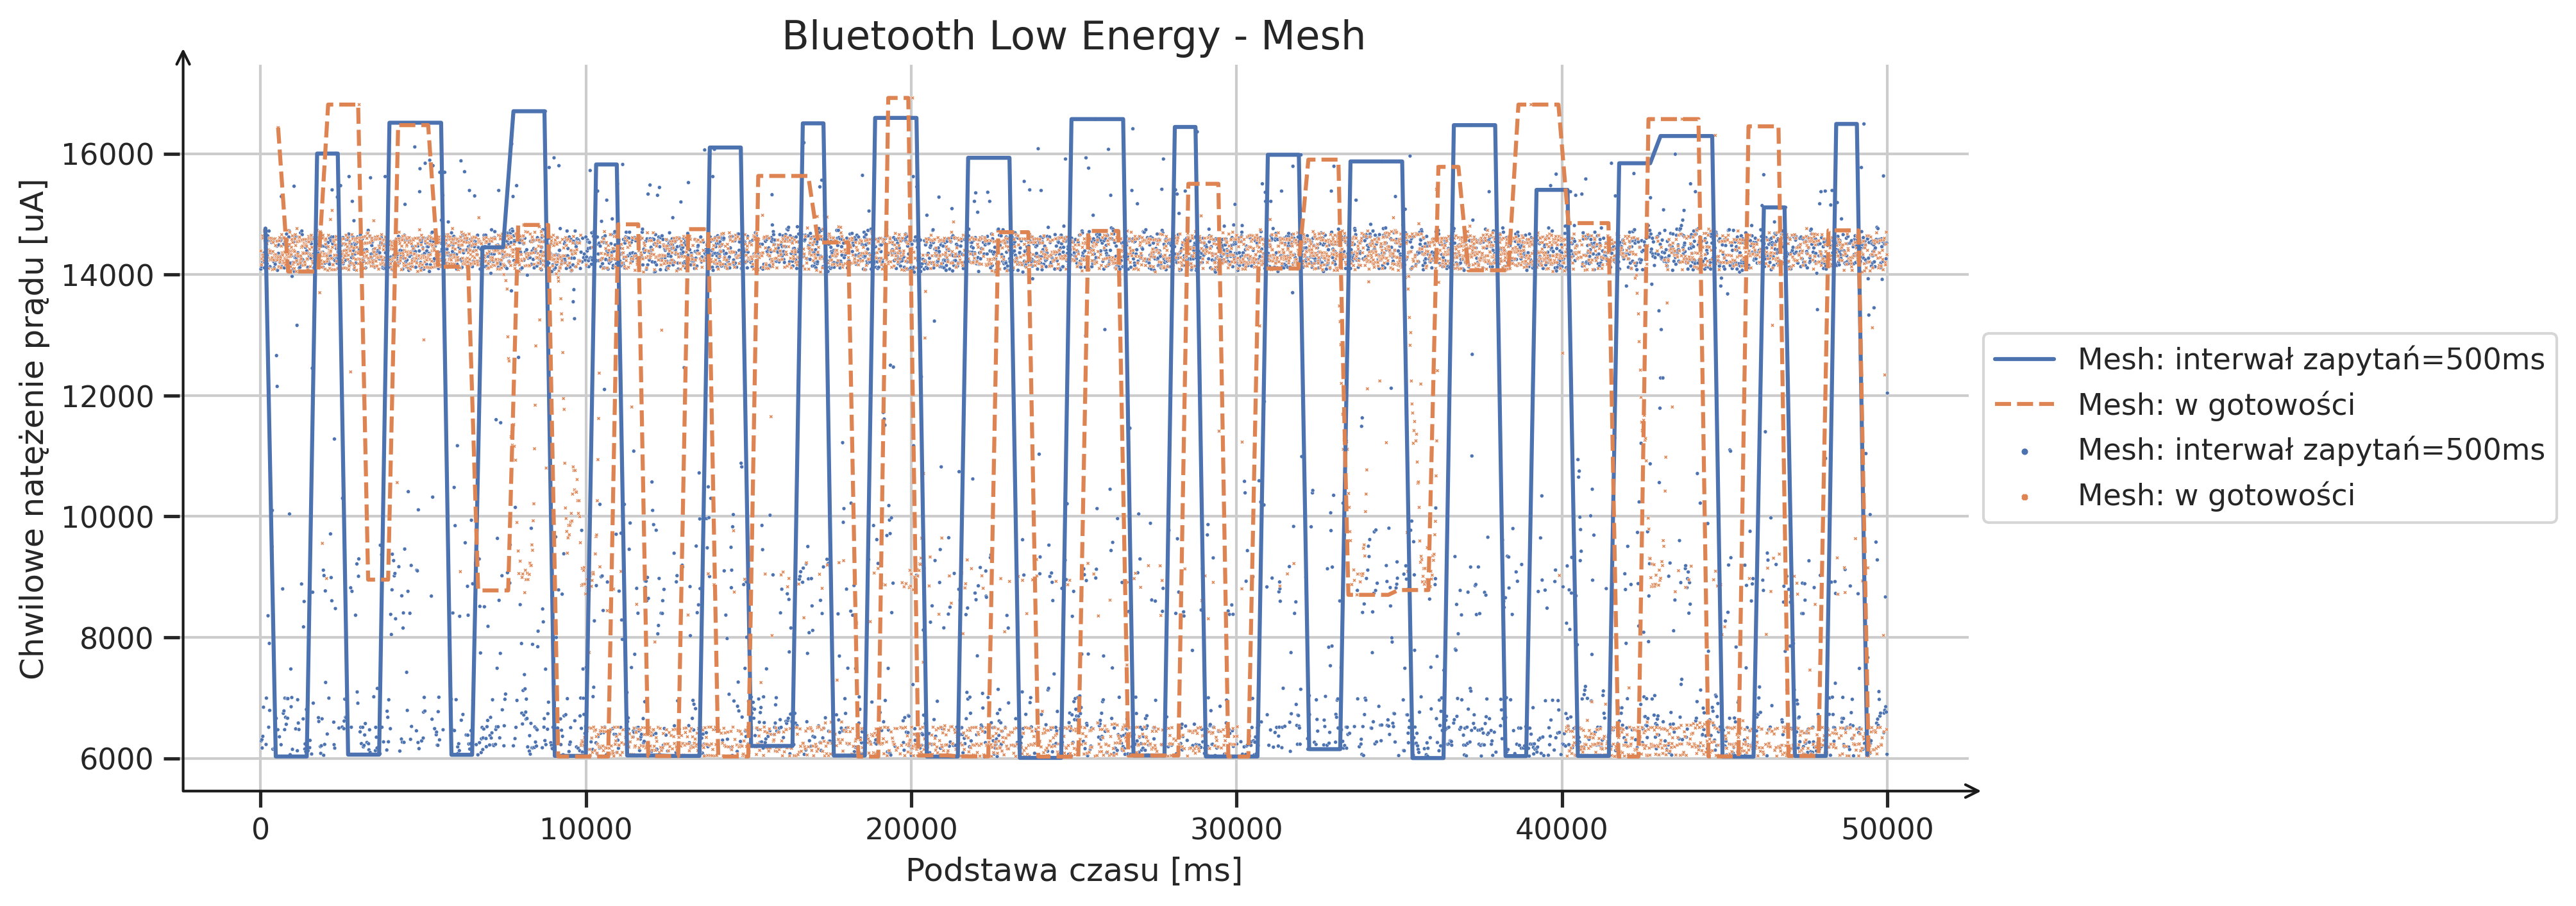
\includegraphics[width=0.99\linewidth]{power_ble_mesh_amps_no_led.png} 
	\caption{Charakterystyka czasowa poboru prądu dla BLE Mesh i modelu Generic OnOff}
	\label{rys:power_ble_mesh_amps}
\end{figure}

\lipsum[1-3]
\begin{figure}[!htb]
	\centering 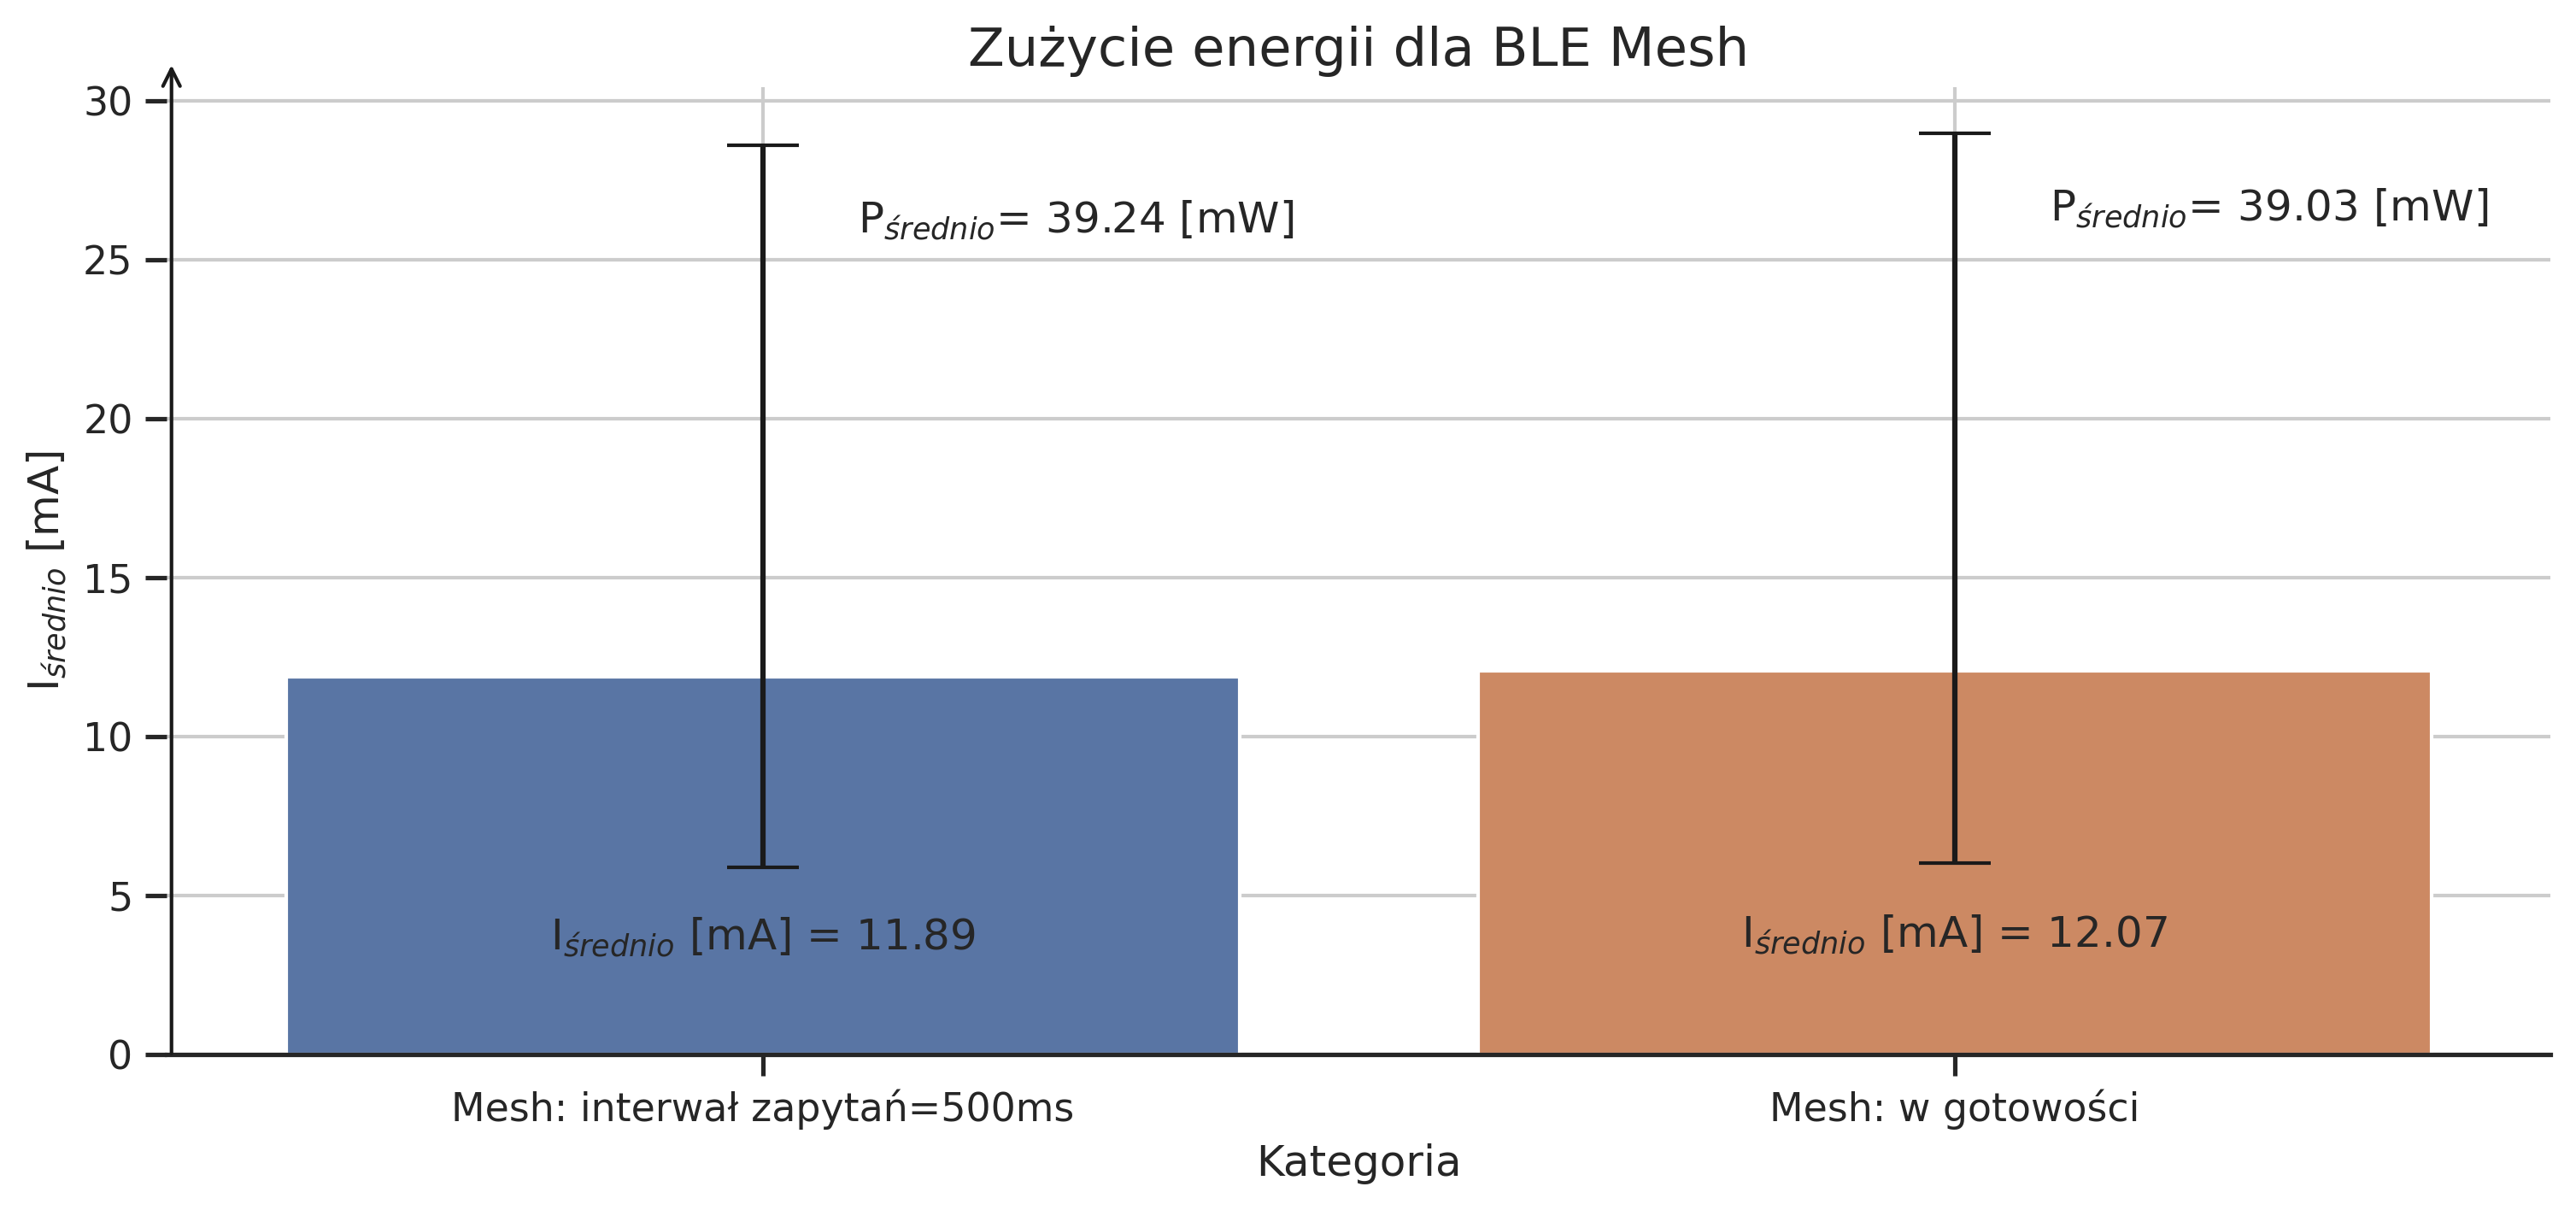
\includegraphics[width=0.99\linewidth]{power_ble_mesh_amps_usage_juxtaposition_no_led.png} 
	\caption{Zestawienie zużycia prądu dla BLE Mesh w zależności od trybu działania}
	\label{rys:power_ble_mesh_amps_usage_juxtaposition}
\end{figure}

\lipsum[1-3]
\begin{figure}[!htb]
	\centering 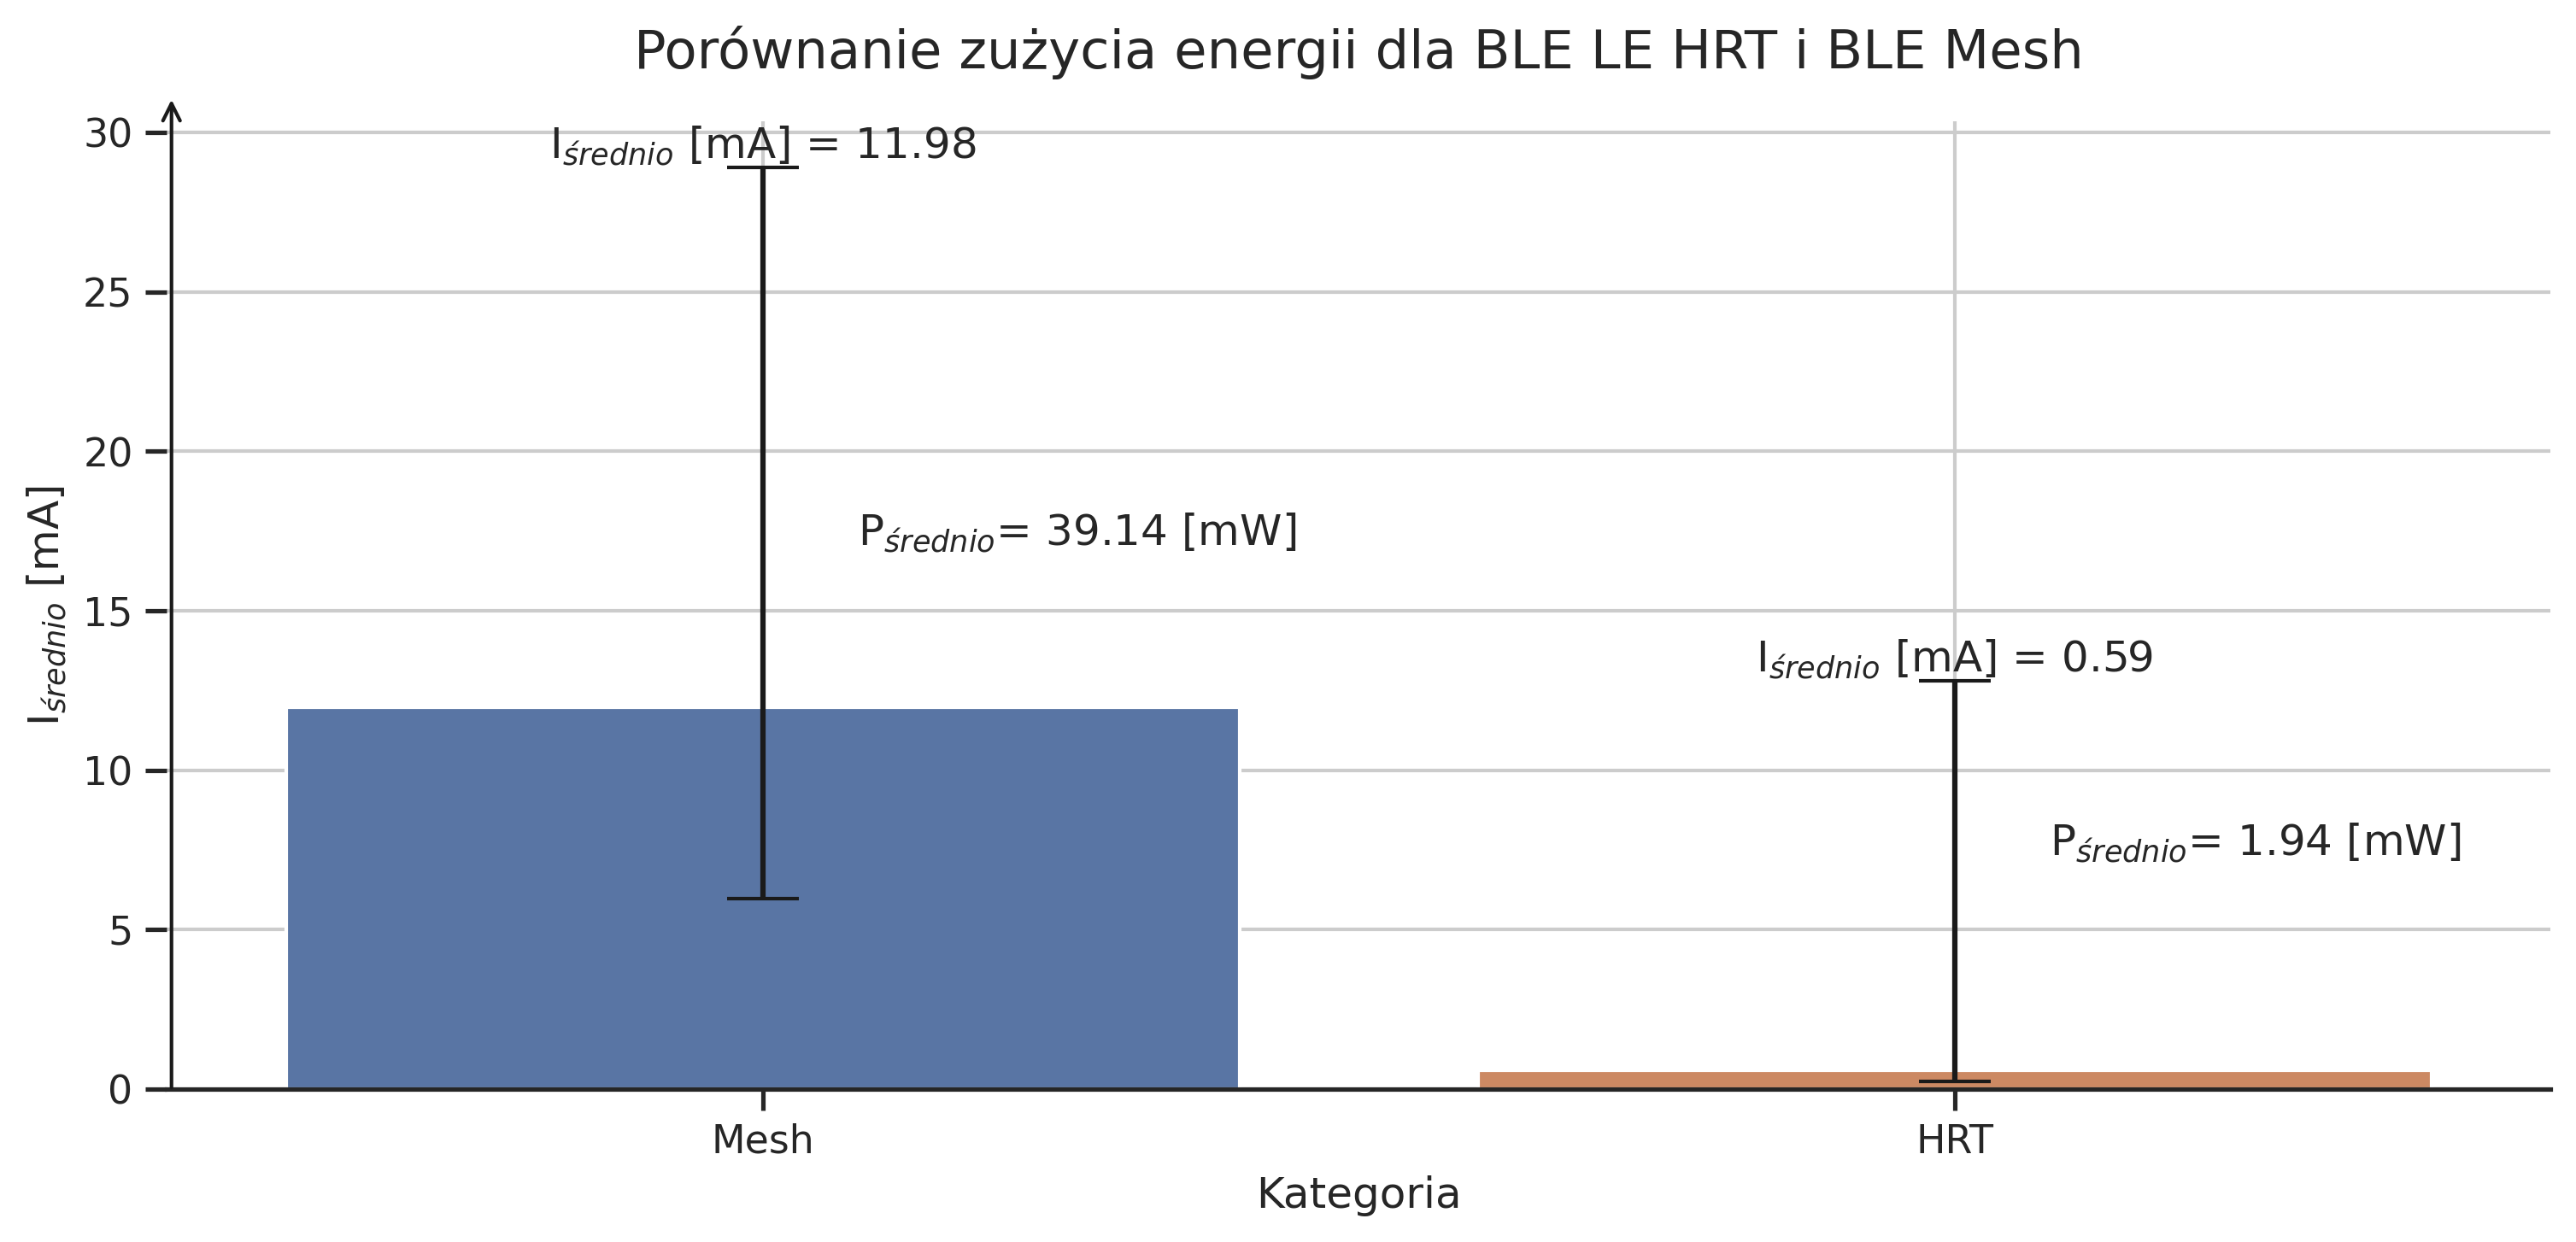
\includegraphics[width=0.99\linewidth]{power_ble_consumption_comparison_no_led.png} 
	\caption{Porównanie średniego zużycia energii pomiędzy BT Low Energy HRT i BLE Mesh}
	\label{rys:power_ble_consumption_comparison}
\end{figure}


